\documentclass{article}

\usepackage{graphicx}
\graphicspath{ {./figures/} }

\usepackage{caption}
\usepackage{subcaption}

\date{\today} % You can replace \today with a specific date if needed

\begin{document}

\begin{center}
	\vspace*{\fill}
	\Huge\textbf{Final report}\par
	\vspace{0.2cm}
	\Large\textbf{Introduction to Embodied Artificial Intelligence}\par
	\vspace{2cm}
	\large\textbf{Filip Lobpreis, Bohdan Kopčák}\par
	\vspace{0.2cm}
	\large\textbf{Group 9}\par
	\vspace{1cm}
	\large\textit{\today}\par
	\vspace*{\fill}
\end{center}

% How you use the 10 pages is up to you, but a reasonable choice
% might be 5 pages focussing on design of mechanical and control
% architecture, 2 pages of design choices and reasons for them, 2 pages
% of evaluation methods and results, and 1 page of discussion and
% conclusions for each part. Don't worry if this structure doesn't
% fit your approach. Use whatever structure that fits, but remember
% the topics you need to cover.

\section{Design development}
\label{sec:development}

\subsection{Mechanical design}
\label{subsec:mechanical_design}

\subsubsection{Early design iterations}

Since the early days of the design, our concern was mainly focused on ability to scale steep surfaces. The traction of
wheels that were available to us was not ideal and the robot tended to slip often in our original design. This led us
to a decision to shift vehicle weight forwards and reduce it as much as possible. Early in the design we also
encountered problems with passing the upper edge of the slope. With our original design with wheels in the back 
the vehicle would get stuck with its center on the edge.

\begin{figure}[!htbp]
	\centering

	\begin{subfigure}{\textwidth}
		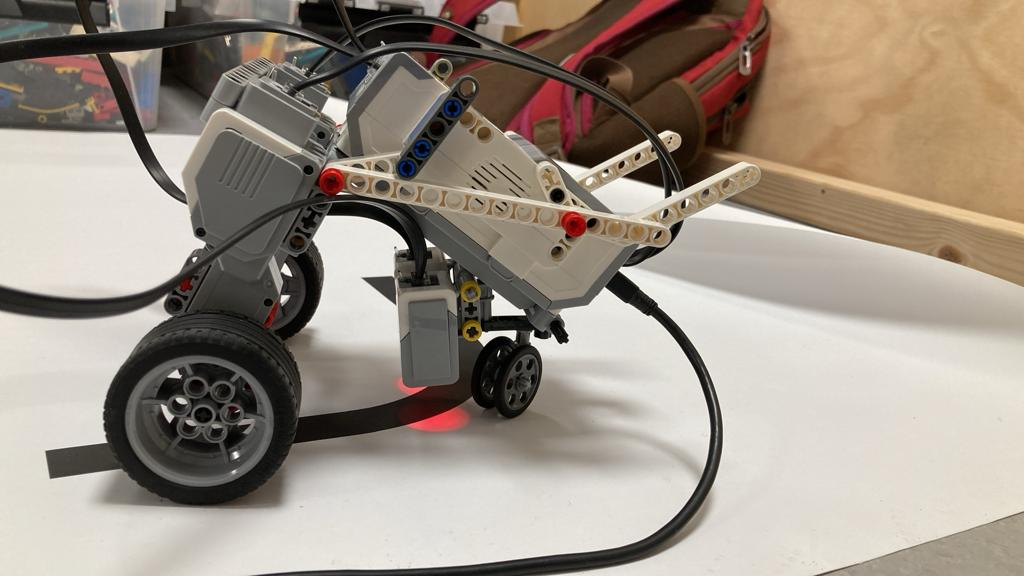
\includegraphics[width=\textwidth]{./figures/old-v-shape.jpeg}
		\caption{Original V shape design}%
	\end{subfigure}
	
	\vspace{\baselineskip}

	\begin{subfigure}{0.48\textwidth}
		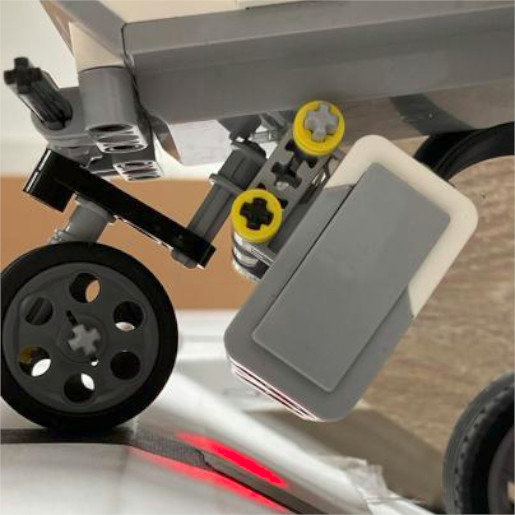
\includegraphics[width=\textwidth]{./figures/old-coaster-wheel.jpeg}
		\caption{Sensor placement detail}%
	\end{subfigure}
	\hfill
	\begin{subfigure}{0.48\textwidth}
		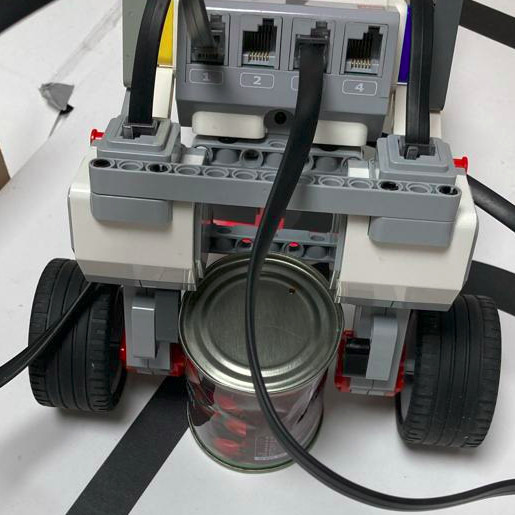
\includegraphics[width=\textwidth]{./figures/old-can-placement.jpeg}
		\caption{Convenient can area}%
	\end{subfigure}
	
	\vspace{\baselineskip}

	\begin{subfigure}{\textwidth}
		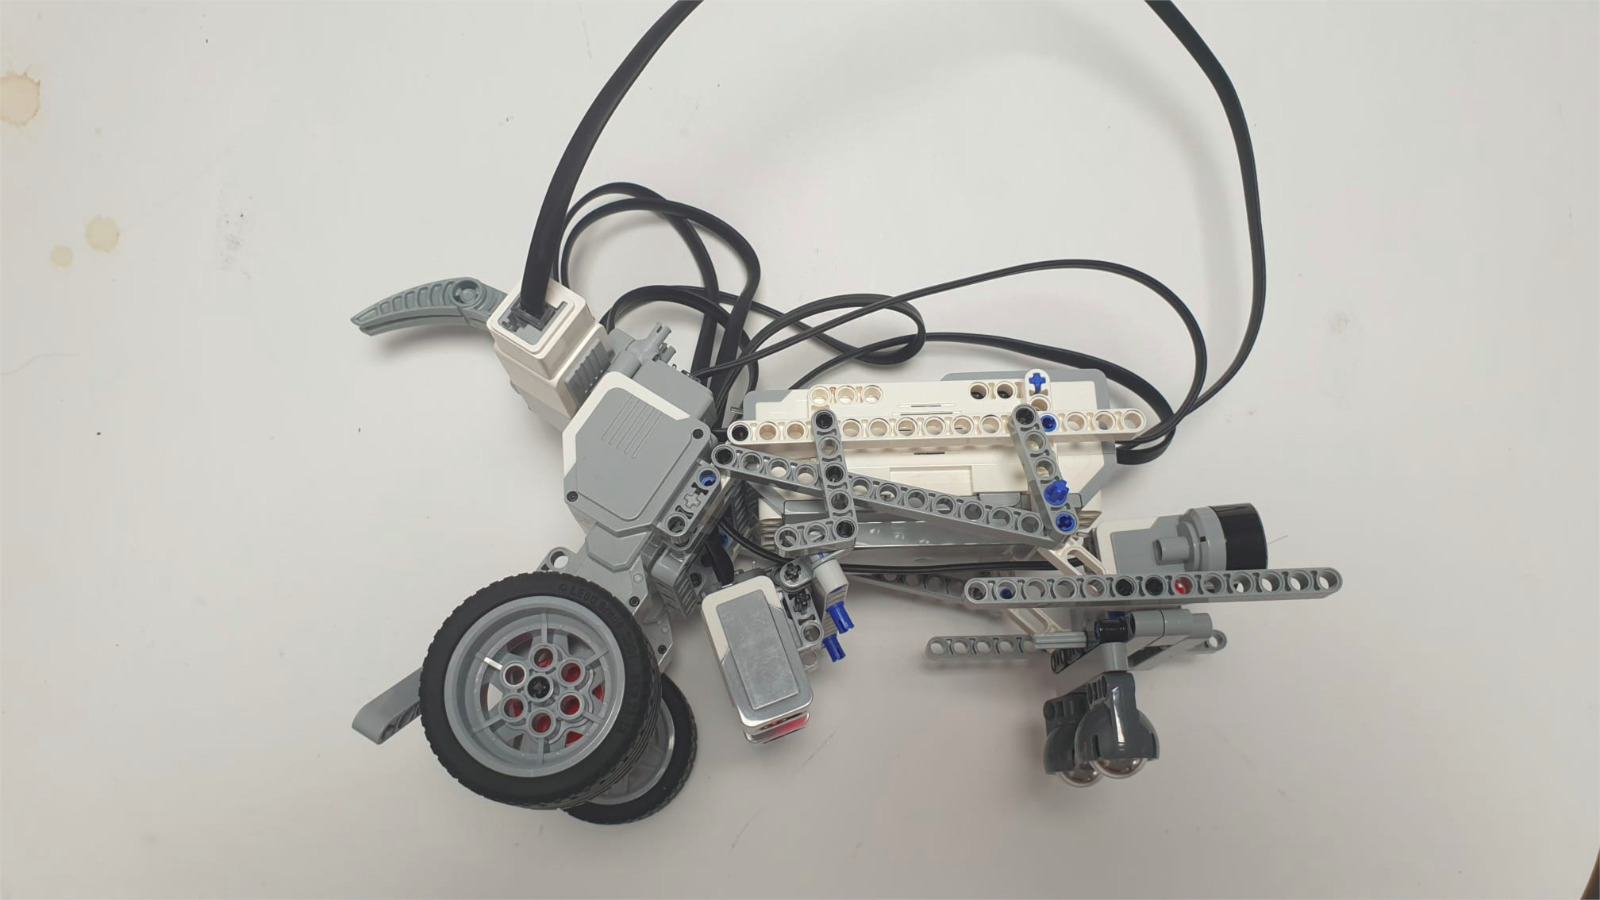
\includegraphics[width=\textwidth]{./figures/new-prototype.jpeg}
		\caption{Newest design iteration}%
	\end{subfigure}

	\caption{Design changes with details}%
    \label{fig:design-changes}%

\end{figure}

\newpage

These factors led us to adapting a V shaped design that we kept through all the subsequent iterations. The design can 
be seen in \ref{fig:design-changes}. This design, with motors and EVO brick forming a V, and with minimal added
structure elements, provided enough ground clearance to pass the slope edge and shifted weight to the front. When on 
the slope, the brick side of the V shape became leveled, providing enough force for the wheels to grip.

Unfortunately, albeit providing improvent in many areas, the design also provided some unexpected challenges.
Because of the V shape, no surface was truly perpendicular to the ground, complicating the placement of line-following
sensors. The sensor placement itself went through multiple design iterations and was a major caveat of our design.
Our rigid body constraints didn't left much room for the sensor placement, resulting in only three possible
configurations -- between motors, below the V and in front of the vehicle.

We initially favoured the second variant mentioned, as it allowed for a convenient can capture mechanism in between
the motors \ref{fig:design-changes}. However, the sensors had to be placed rather high to prevent traversal issues, which meant less
response due to the distance from the surface. Unstable fixation of the sensors (see \ref{fig:design-changes}) led us to seek another
minor redesign, that slightly changed the shape of the V and moved sensors to their final position in the front of the vehicle.

\subsubsection{Final design}

The final design brought many changes to the robot. We have kept the design derictions from our previous design, but
we have changed the the way the motors were fixed to the brick. The new fixation provided more stiffness to the frame,
 so that model didn't have to be calibrated after every transportation or brick charging, and it has

The final design also provided slightly more space between motors, which enabled us to fit in a servo with a claw-latch
mechanism, and also included a more favourable fixation of the ultrasound sensor in the front.

\subsection{Control design}
\label{subsec:control_design}

\subsubsection{Approaches}
\label{subsubsec:approaches}

The first thing we have tried to do was to create a controller for line following. We have tried two approaches.
The first approach was to create a controller that will create a controller for left and right motor separatelly. In
that way we would have two controllers that will controll the wheels based on the input from the sensors. The sensors
followed the \textit{Aggression principal} of \textit{Braintenberg vehicles}. The disadvantage that we had with this
approach was the presence of multiple PID controll parameters. We had to set up the left and right wheel controller so
that their cooperation would be sufficient for line following.

The second approach was to create a \textit{differential drive}. For this we needed to have the distance between the
points of the wheels that touched the ground, radius of the wheels. For this approach we needed only one PID controller.
The difference with the previous approach is that the previous approach changes the speed of the motors and with that
it turns and the differential drive approach uses PID to change the turning rate where the forward speed is kept to be
the same.

All in all, we decided to go with the approach of \textit{differential drive} because of the reason, that it required
less parameters to set up. Every time we came to the laboratory we had to set up the parameters again and with every
modification of the mechanical structure (mentioned in \ref{subsec:mechanical_design}) we had to adjust the parameters.
That is why we decided to go with less parameters.

\subsubsection{Contol}
\label{subsubsec:control}

In our final implementation of the control of the robot we have finished with a schema that is displayed on
Fig.~\ref{fig:controlDiagram}.

\begin{figure}[hpbt!]
	\begin{center}
		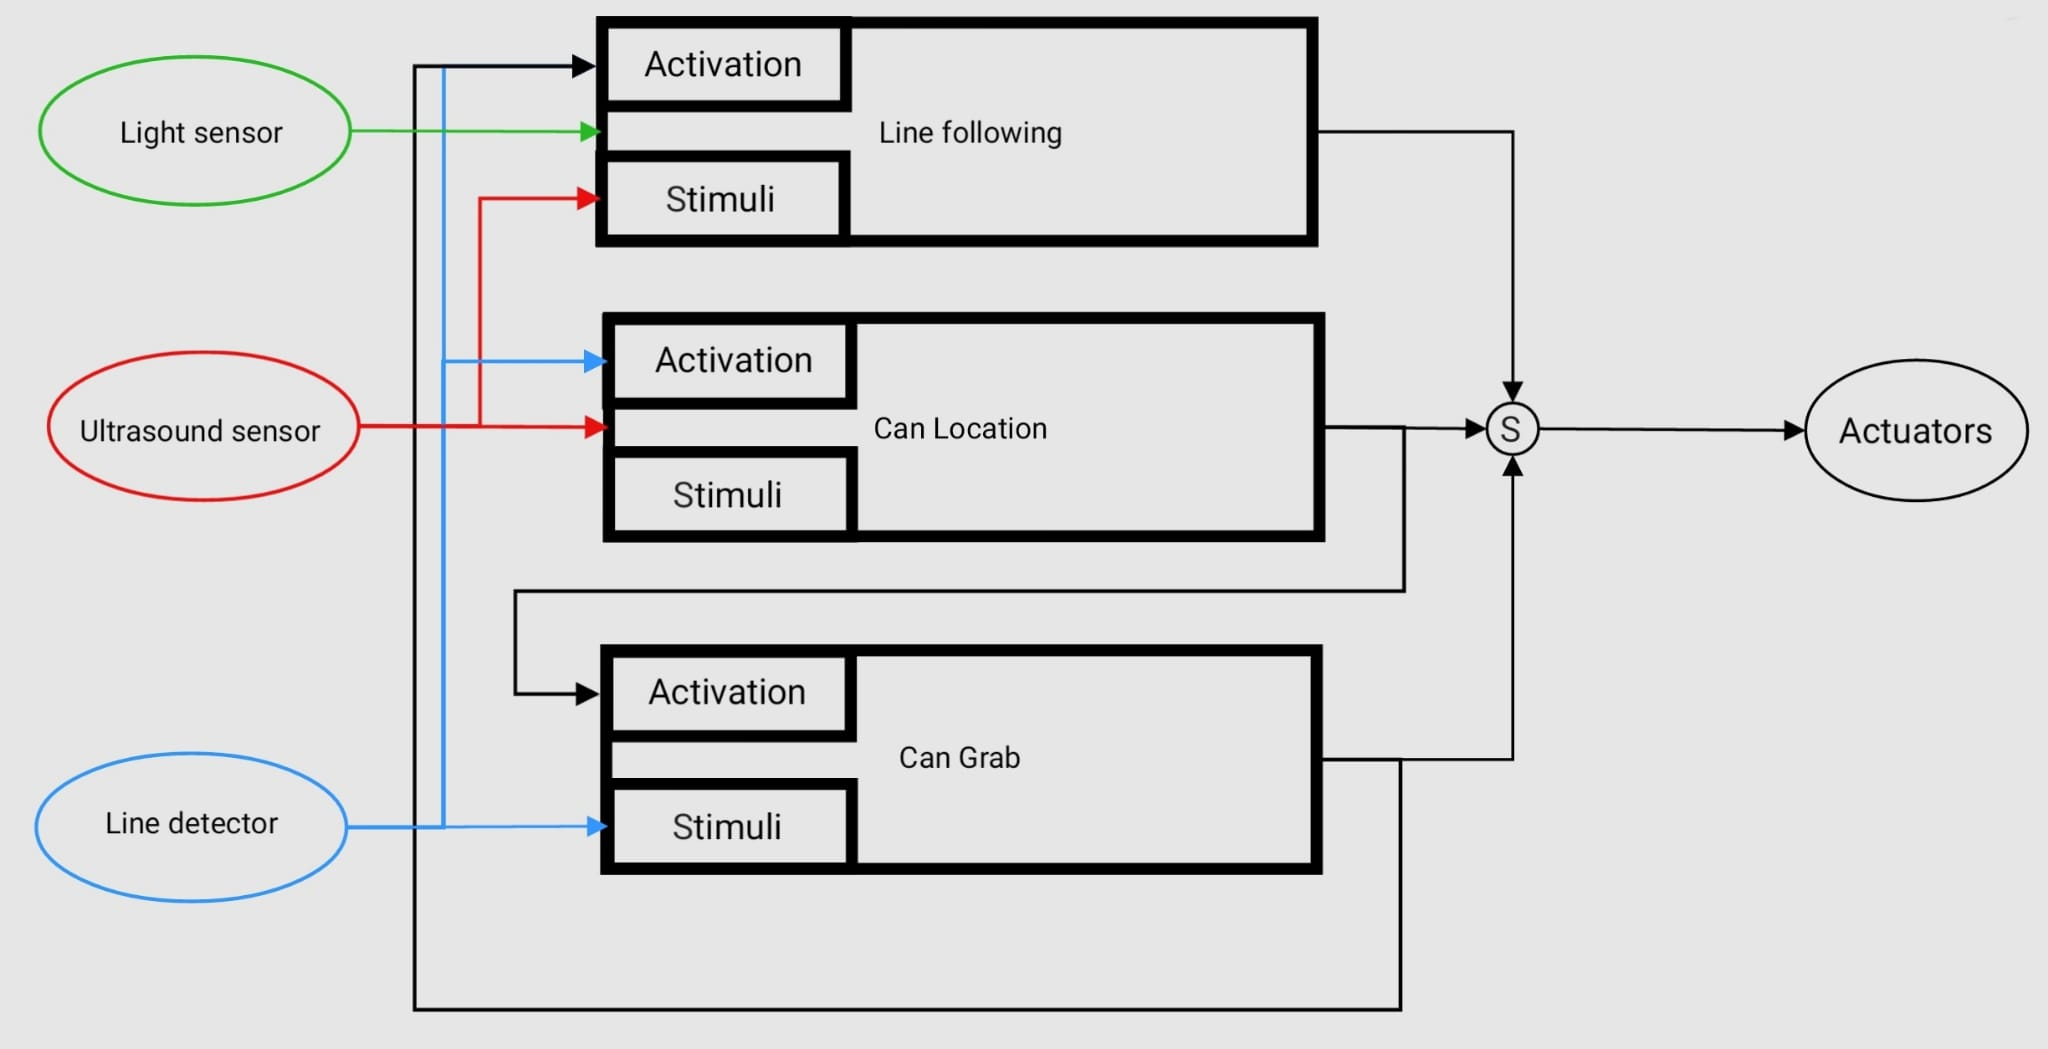
\includegraphics[width=0.95\textwidth]{"./figures/ControlDiagram.jpeg"}
	\end{center}
	\caption{The control diagram for the robot.}
	\label{fig:controlDiagram}
\end{figure}

We had three main behaviours:
\begin{itemize}
	\item Line following - behaviour that takes input from \textit{Light sensors} and uses it in PID controller.
	\item Can locating - behaviour that will take multiple values from the surrounding and based on the input
						 detects the can.
	\item Can grabbing - 
\end{itemize}

We had three inputs from sensors:
\begin{itemize}
	\item Light sensors - sensors detecting, wether we are follwing the line correctly. We used reflection function
		  to get the input from both of them,
	\item Ultrasound sensor - sensor that is scanning the change of distances in front of the robot, so that we can
		  detect the can,
	\item Line detector (Color sensor) - sensor used for end of line detection. This sensor was used as an activation
		  function for jumping between the sates of \textit{Line following} and \textit{Can location}.
\end{itemize}

The output\textit{Actuators} is ment to be the left and right motor and the gripper. The state we are currently in takes
full control of all the motors at the same time.

The line following is activated either by \textit{Line detector} when it finds a line or by the finished operation
of \textit{Can grabbing}. It is stimulated by the ultrasound detection. This signal at the same time is used as an
input to the \textit{Can localization} behaviour. This behaviour is activated by loosing the line. In this behaviour
we make an initial turn to the left and we scan the distance from the robot from the ultrasound sensor. This we store
in memory and do a first derivation of the measured data. We knew that the can will be located at least 10 cm from the
wall, that is why we tried to detect the change of more then 10 cm. This approach was a bit troublesome on the lower
platform where there was no wall, so we limited the difference by 25 cm. The last state \textit{Can grabbing} is activated
by the output of the \textit{Can localization}, here if we found the can we turned arround and grabbed the can with
the gripper as mentioned in%~\ref{subsubsec:grabbing}.

\subsubsecion{PID controller}
\label{subsubsec:pid}

For the line following we have decided to use PID controller.

\section{Evaluation methods and results}
\label{sec:evaluation_methods_and_results}



\section{Discussion and conclusions}
\label{sec:discussion_and_conclusions}



%The robot's behavior-based architecture is shown in Figure~\ref{fig:behaviour_graph}. The basic robot's behaviour will
be avoiding walls, in that sense when the robot will go up the ramp with higher speed the robot will not hit the wall and
potentially destroy itself or the wall.

The next layer of the behaviour will be line following. The robot will follow the line and will try to find the can at
the end of the line.

When an object in front of the robot is detected by the ultrasound sensor, the robot will stop and determine if the
object is a wall or a can. If the object is a can, the robot will try to grab it and then go back to the starting point.

The first floor of the maze will be explored by the robot in the same way as the ground floor. The robot will follow the
line to the can and after grabbing it, it will go back to the ramp either with a straight line or by following the line.

% \begin{figure}[!htbp]
% 	\begin{center}
% 	\vspace{2cm}
% 		\includegraphics[width=0.95\textwidth]{./figures/Behavioral.jpeg}
% 	\end{center}
% 	\caption{Behavioral graph of the designed mobile robot}
% 	\label{fig:behaviour_graph}
% \end{figure}

\section{Physical Structure of the Robot}

We do not have any special requirements on the robot's physical structure. The only factors we had to take in
consideration was robot's ability to climb slopes and to grab the can.

The robot is a standard differential drive robot equipped with two color sensors and a an ultrasound sensor.

We have designed a special passive gripper that is triggered by an impact of the can.

\section{Reliability factors}

The first factor that will affect the reliability of the execution will be line following. We need to make sure that we
will follow the line as precisely as possible and at the same time we want to maintain the speed of the robot on some
higher level.

The other issue will be with changing the states of the robot's behaviour. For example when we miss the can with the passive gripper
we might not have another chance to grab it in the specified time.

We will definitely try to optimise the line following algorithm and also the possibility to change the speed of the
actuators at the ramp.

\section{Testing}

The testing will be done in the following way. We will first test the line following algorithm on the ground floor of
the maze. We will also test if the robot will not hit the wall while following the line.

The other thing that we will be testing is the ability of the robot to climb the ramp. We will test the speed of the
wheels and adjust them accordingly. The factor that will affect the ability to climb the ramp is the weight distribution
of the robot. If we find out that the distribution is not optimal and is in a way of completing the task, than we will
change the robot design.

The next thing that we will test is the grabbing mechanism. The current implementation needs a bit of force to passively
close the gripper. That may not be the best solution, so we will test the gripper and if we find out that it is not
possible to grab the can, we will change our approach.

The robot's performace will be measured by time. We will measure the time it takes to complete the task and we will try
to optimise it.

\end{document}

